\begin{figure*}[htbp]
\begin{subfigure}{0.48\textwidth}
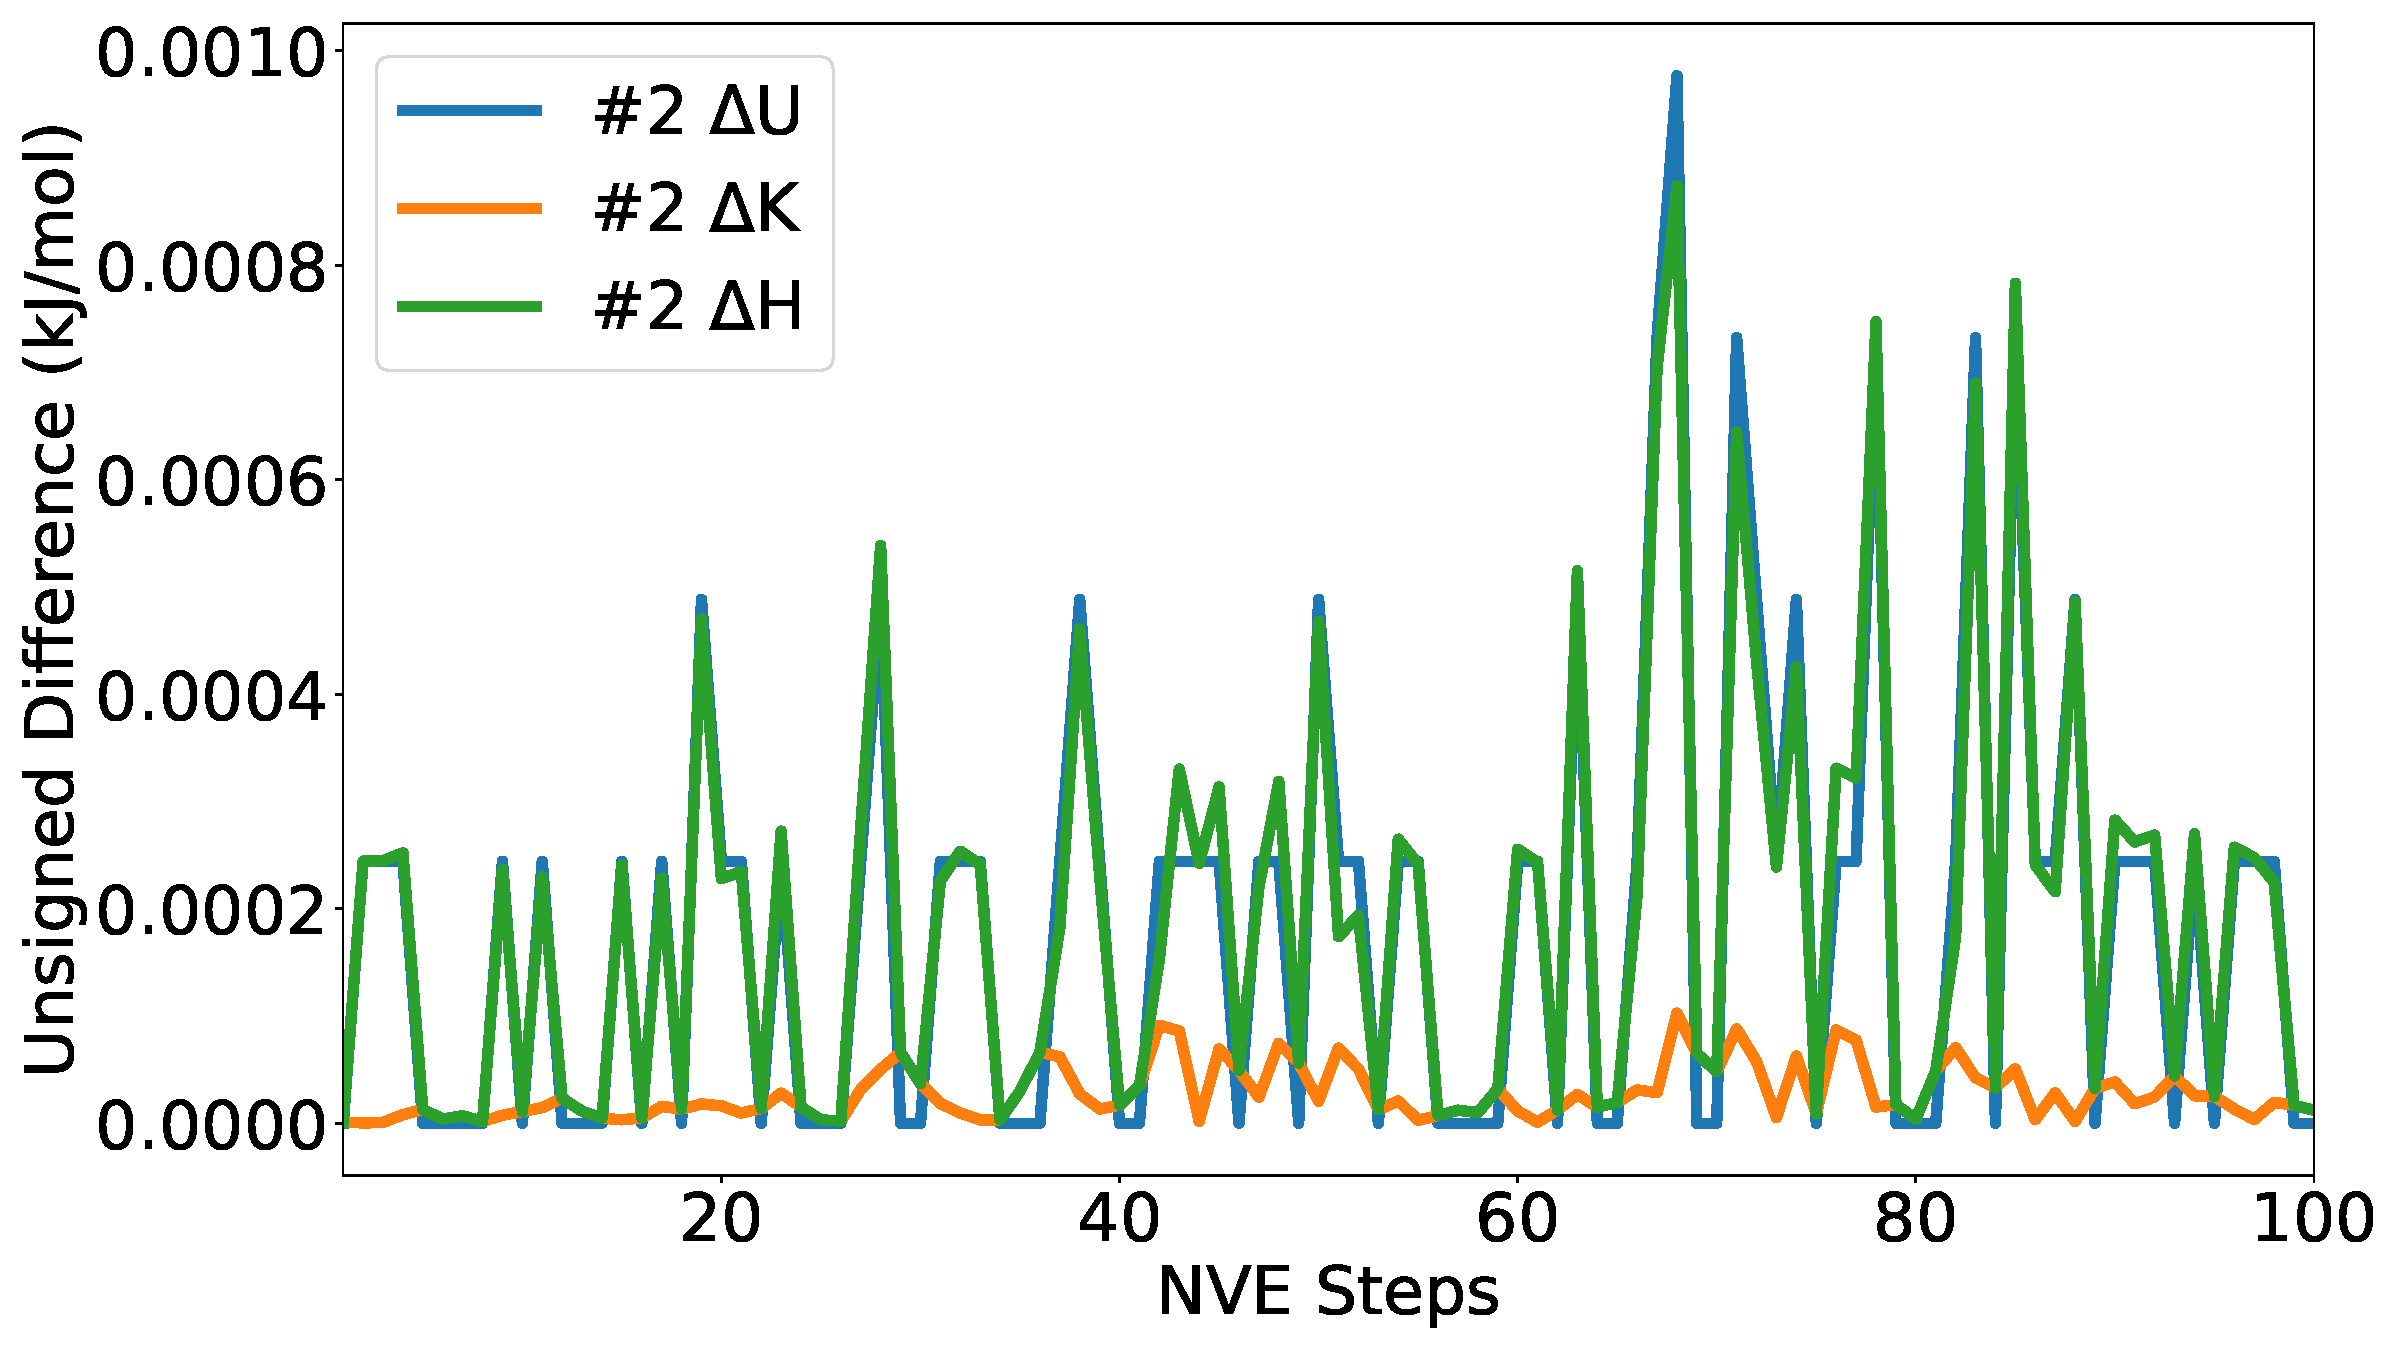
\includegraphics[width=\linewidth]{figs/div2.pdf}
\end{subfigure}
\\
\begin{subfigure}{0.48\textwidth}
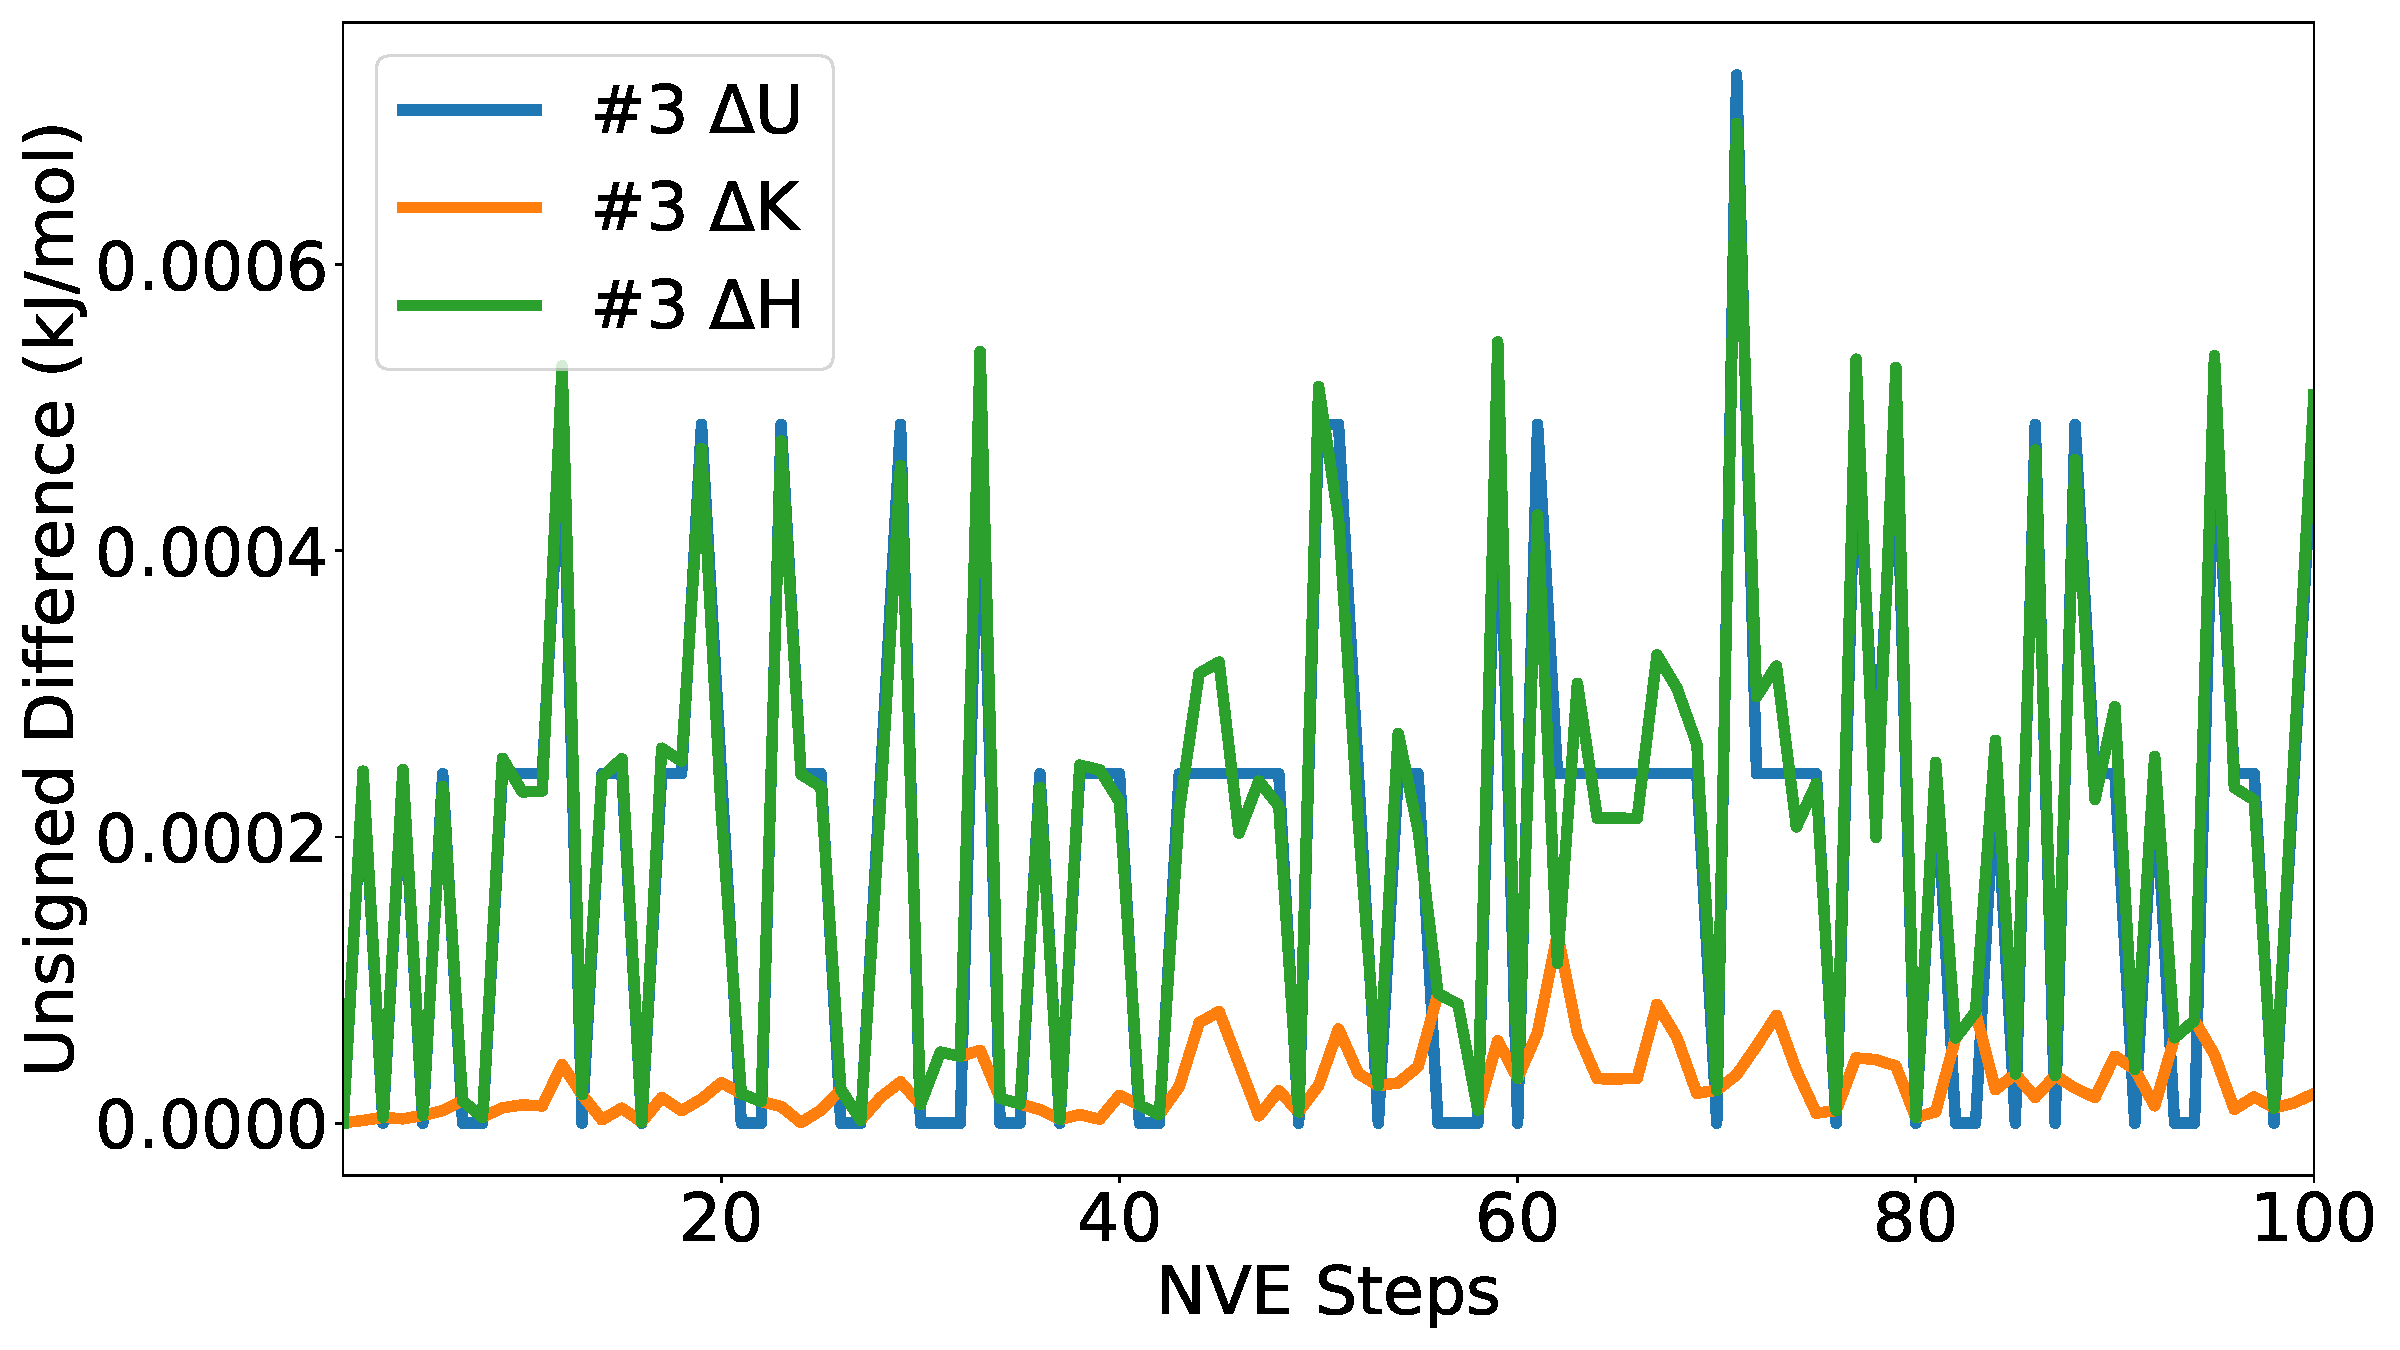
\includegraphics[width=\linewidth]{figs/div3.pdf}
\end{subfigure}
\begin{subfigure}{0.48\textwidth}
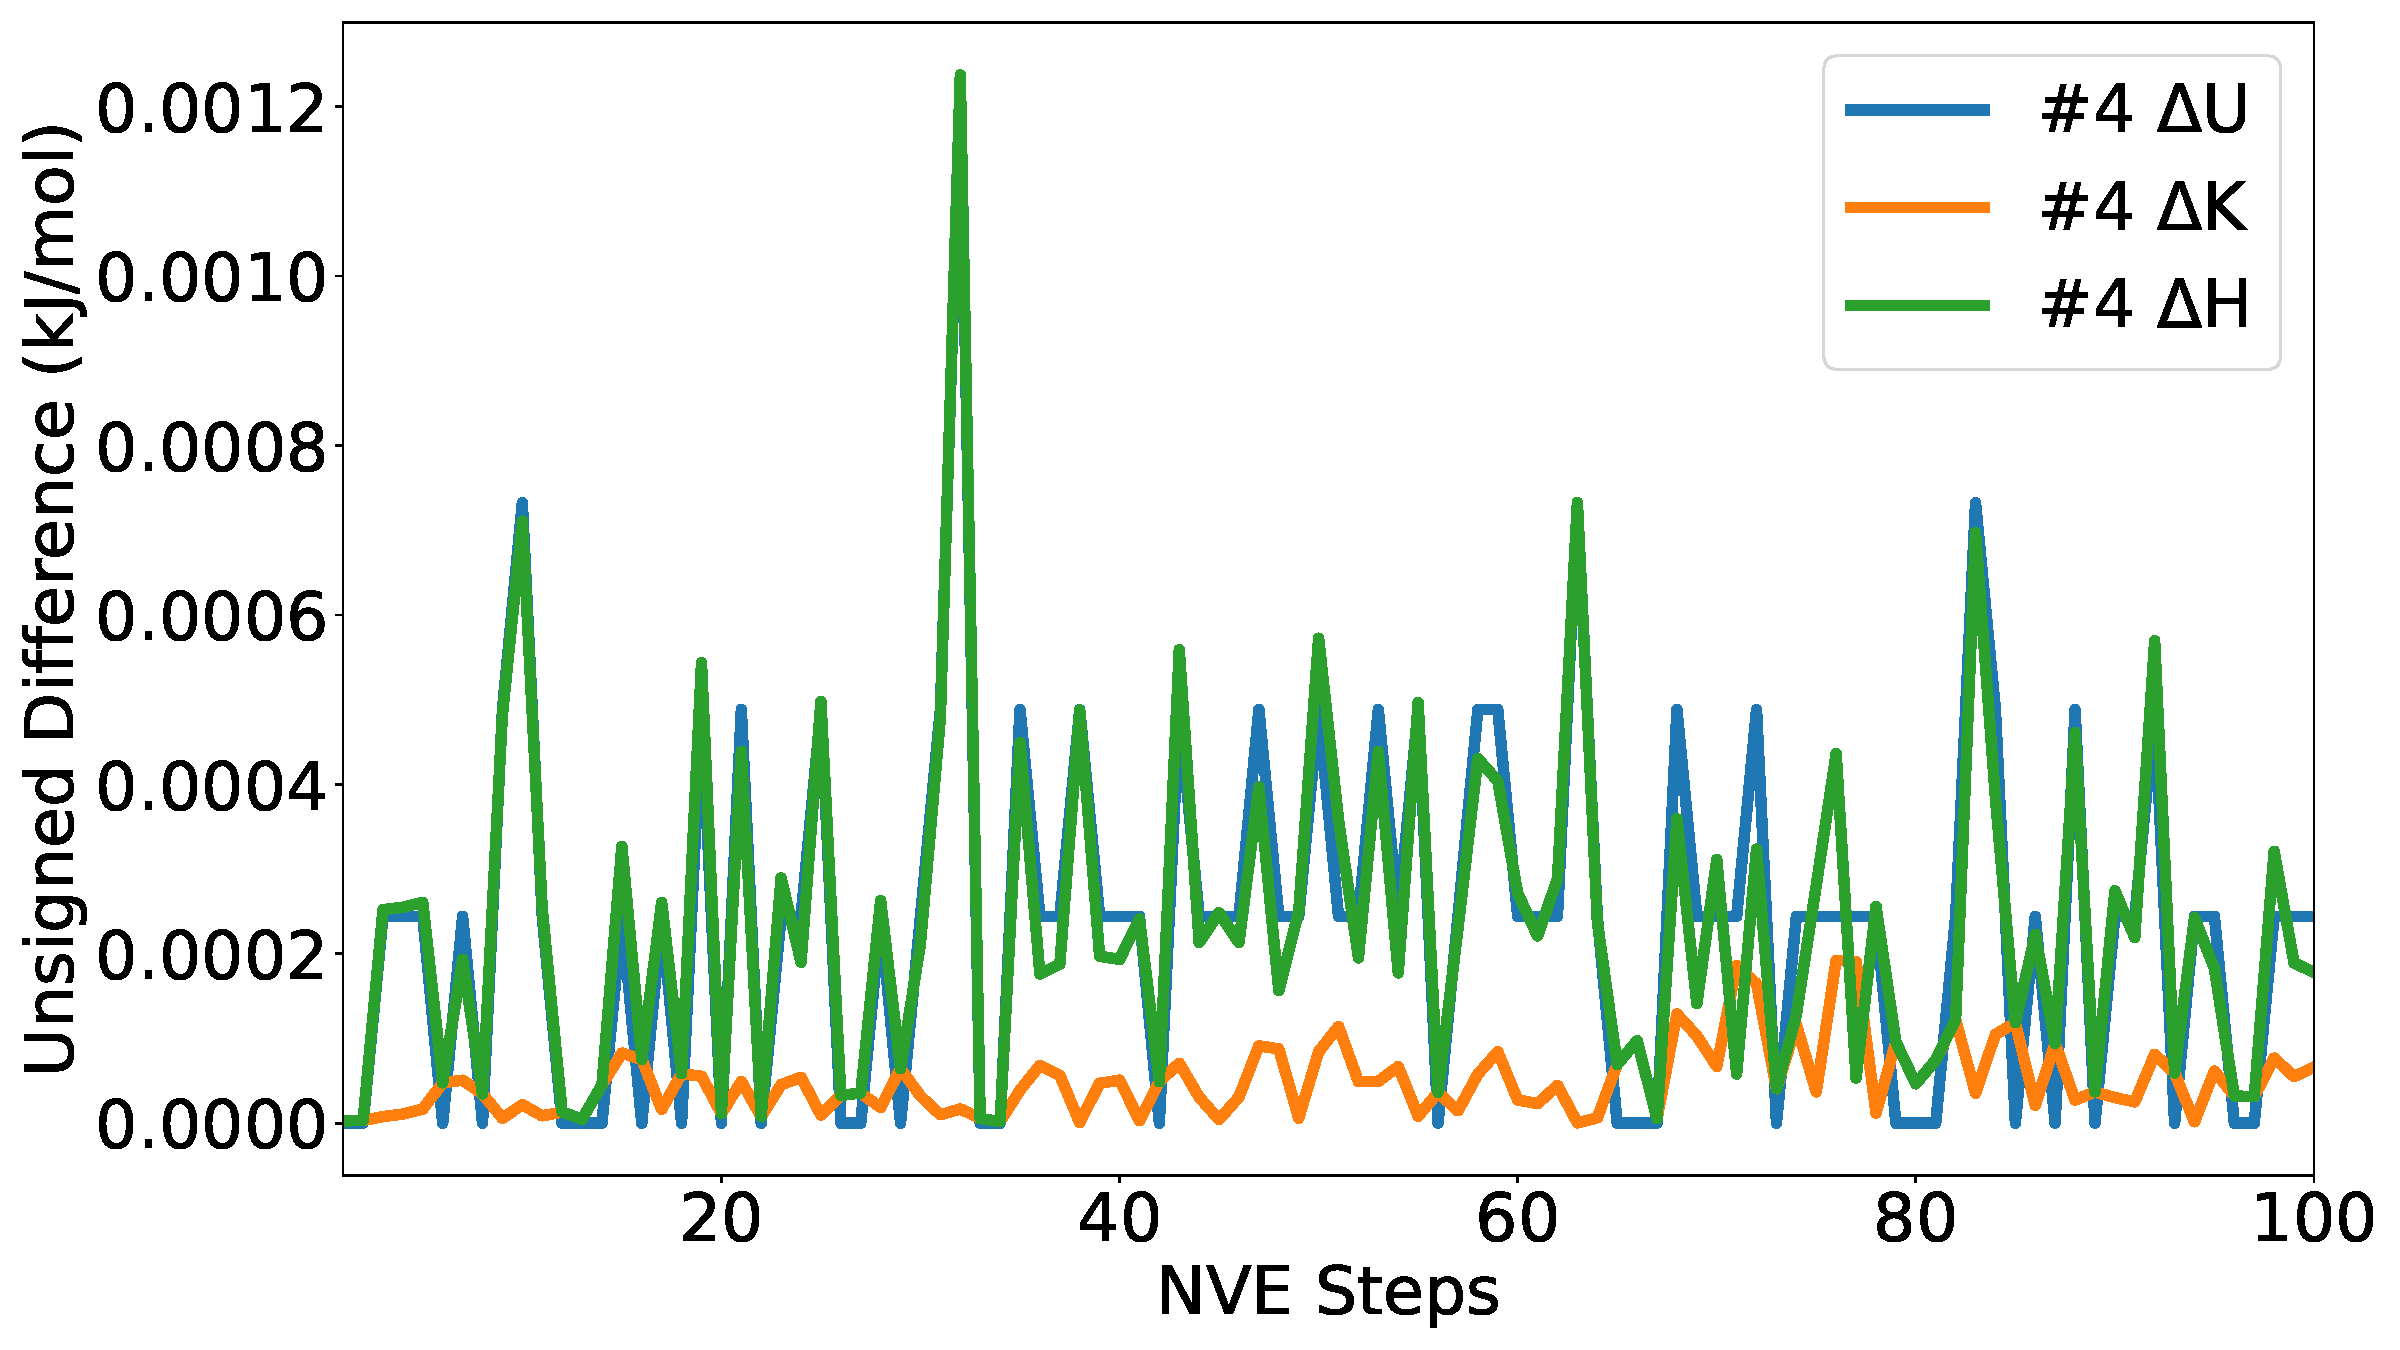
\includegraphics[width=\linewidth]{figs/div4.pdf}
\end{subfigure}
\\
\begin{subfigure}{0.48\textwidth}
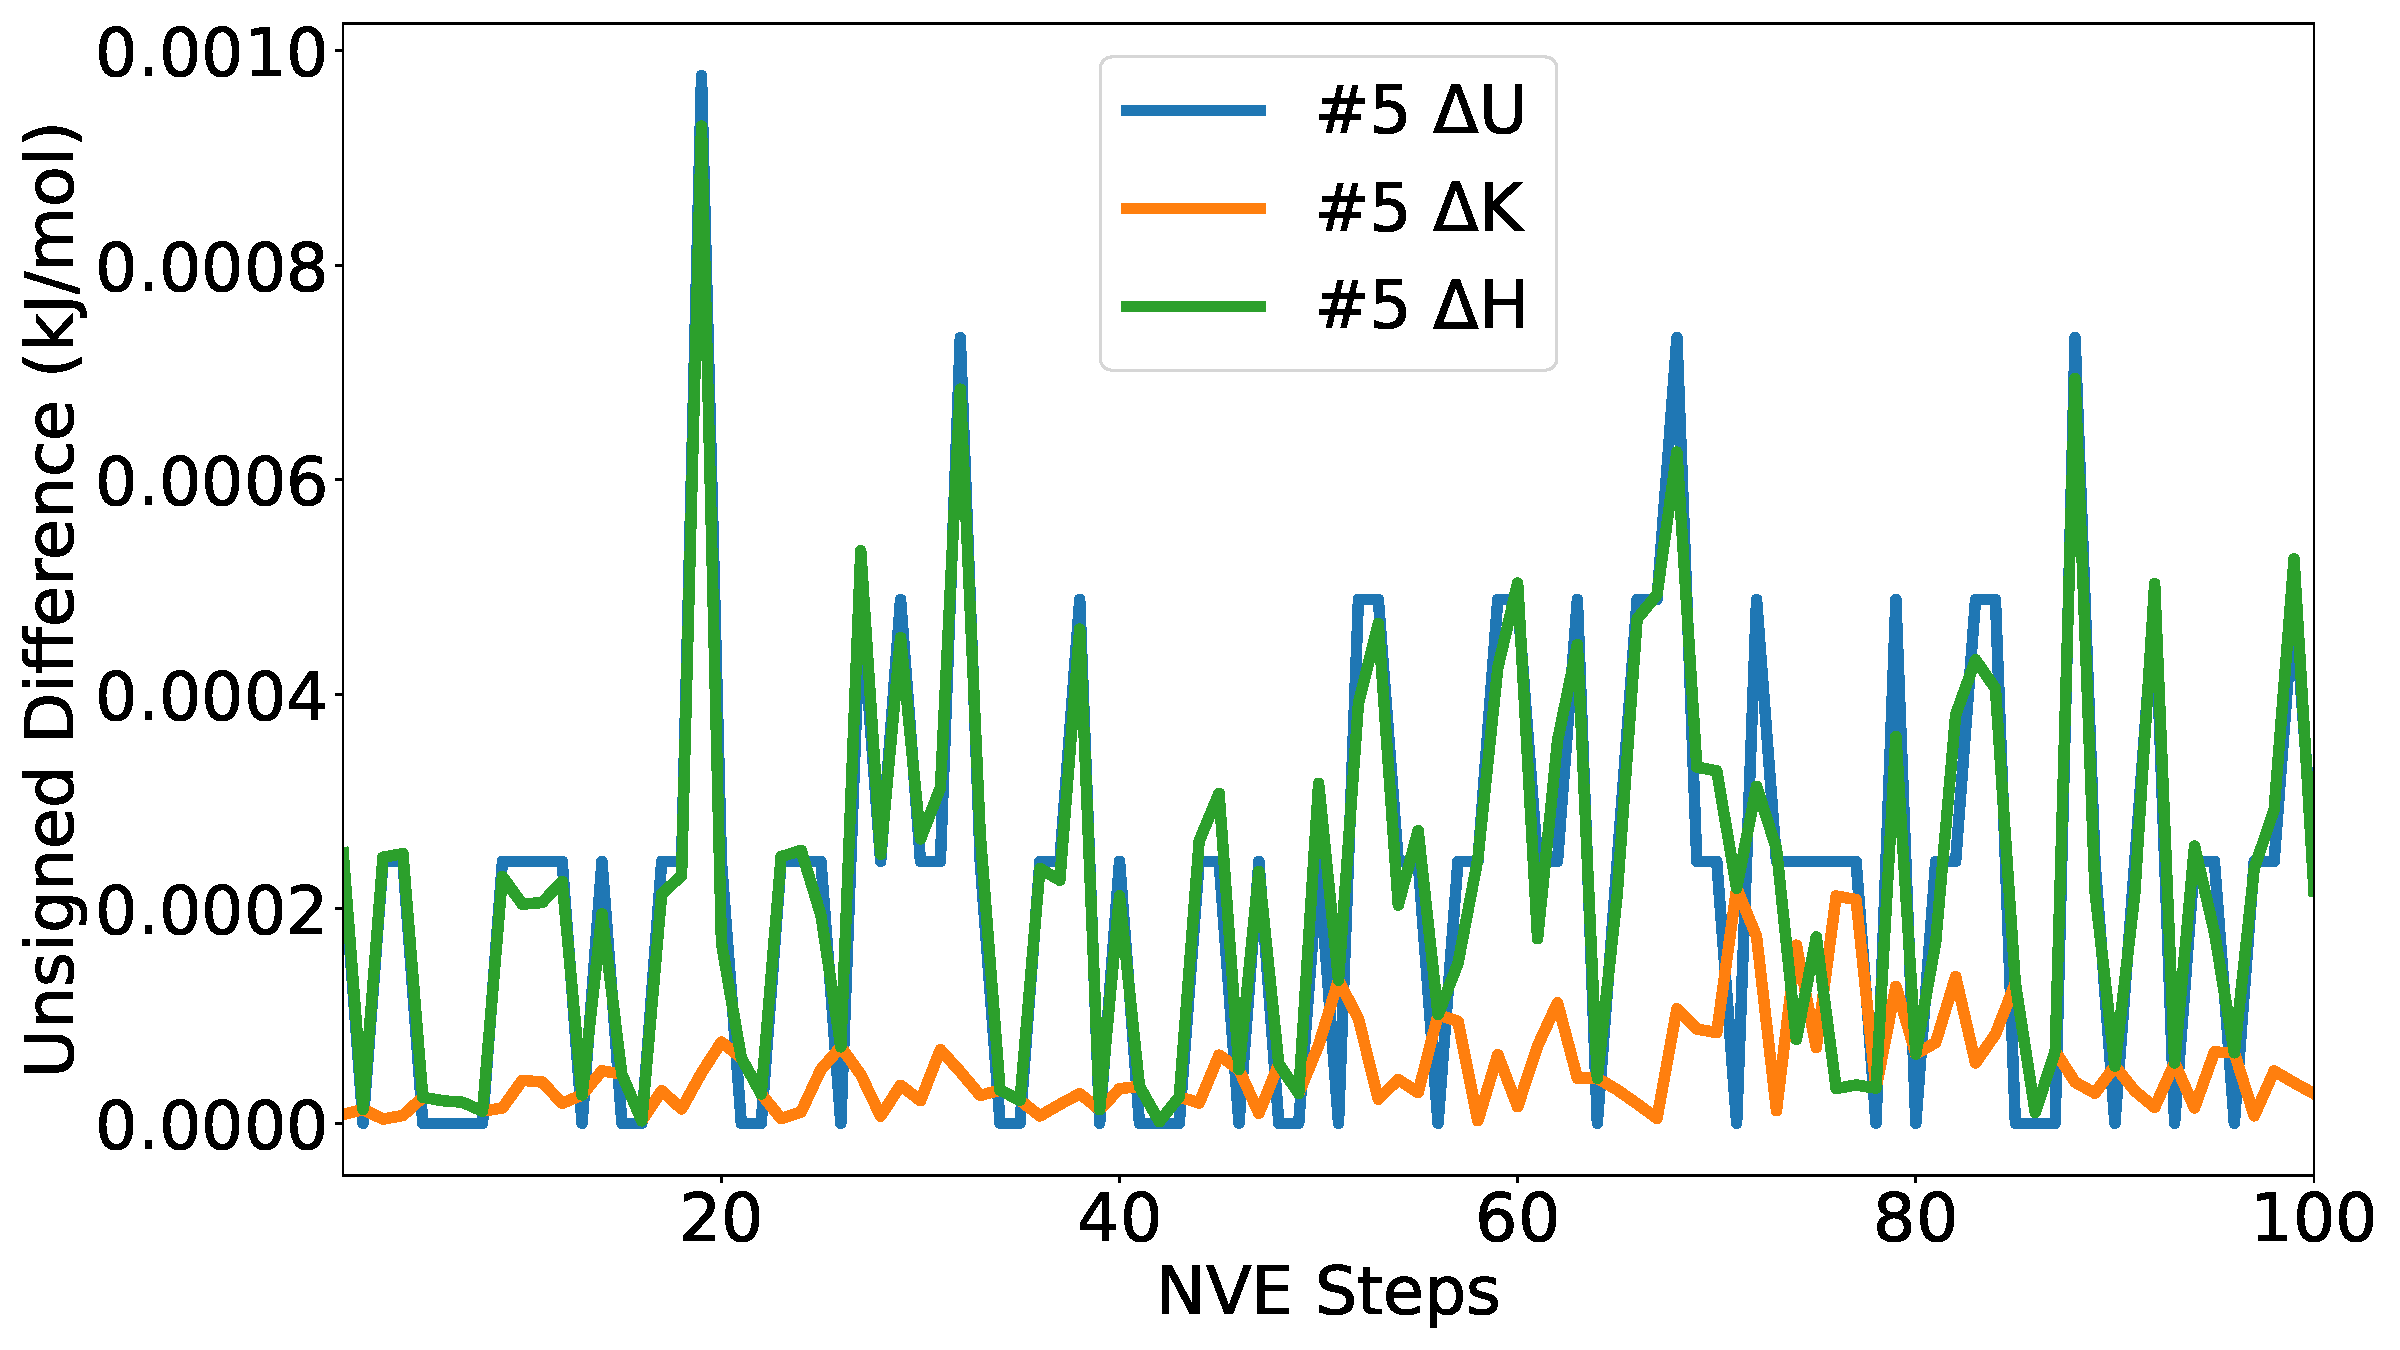
\includegraphics[width=\linewidth]{figs/div5.pdf}
\end{subfigure}
\begin{subfigure}{0.48\textwidth}
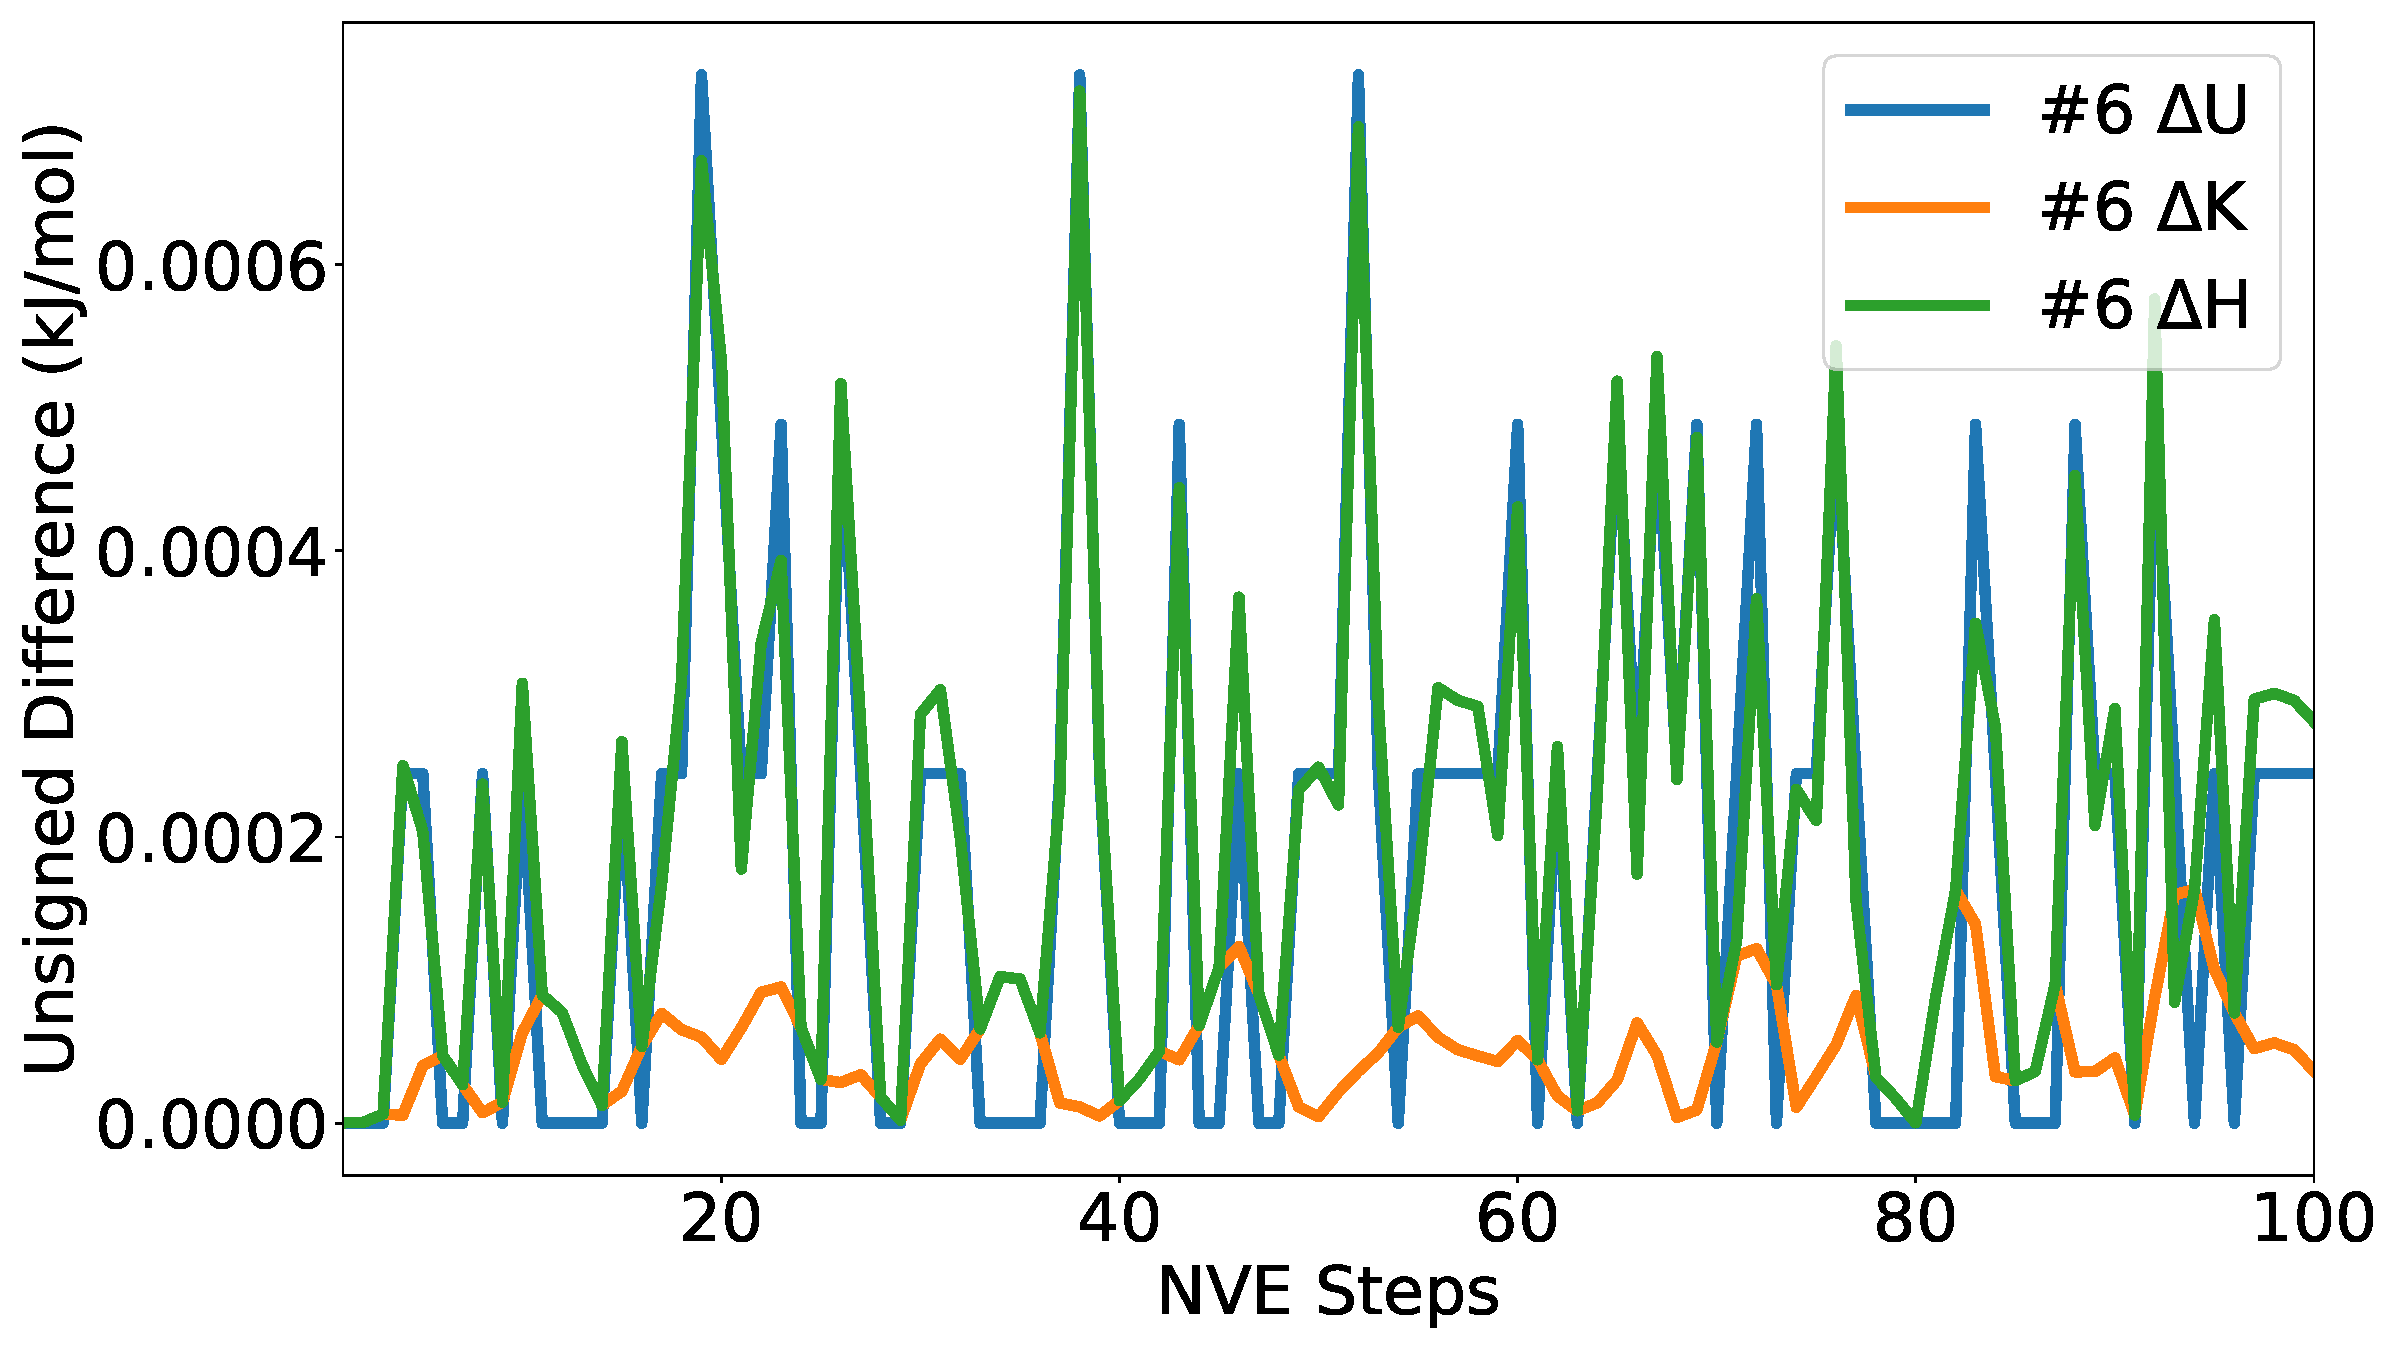
\includegraphics[width=\linewidth]{figs/div6.pdf}
\end{subfigure}
\\
\begin{subfigure}{0.48\textwidth}
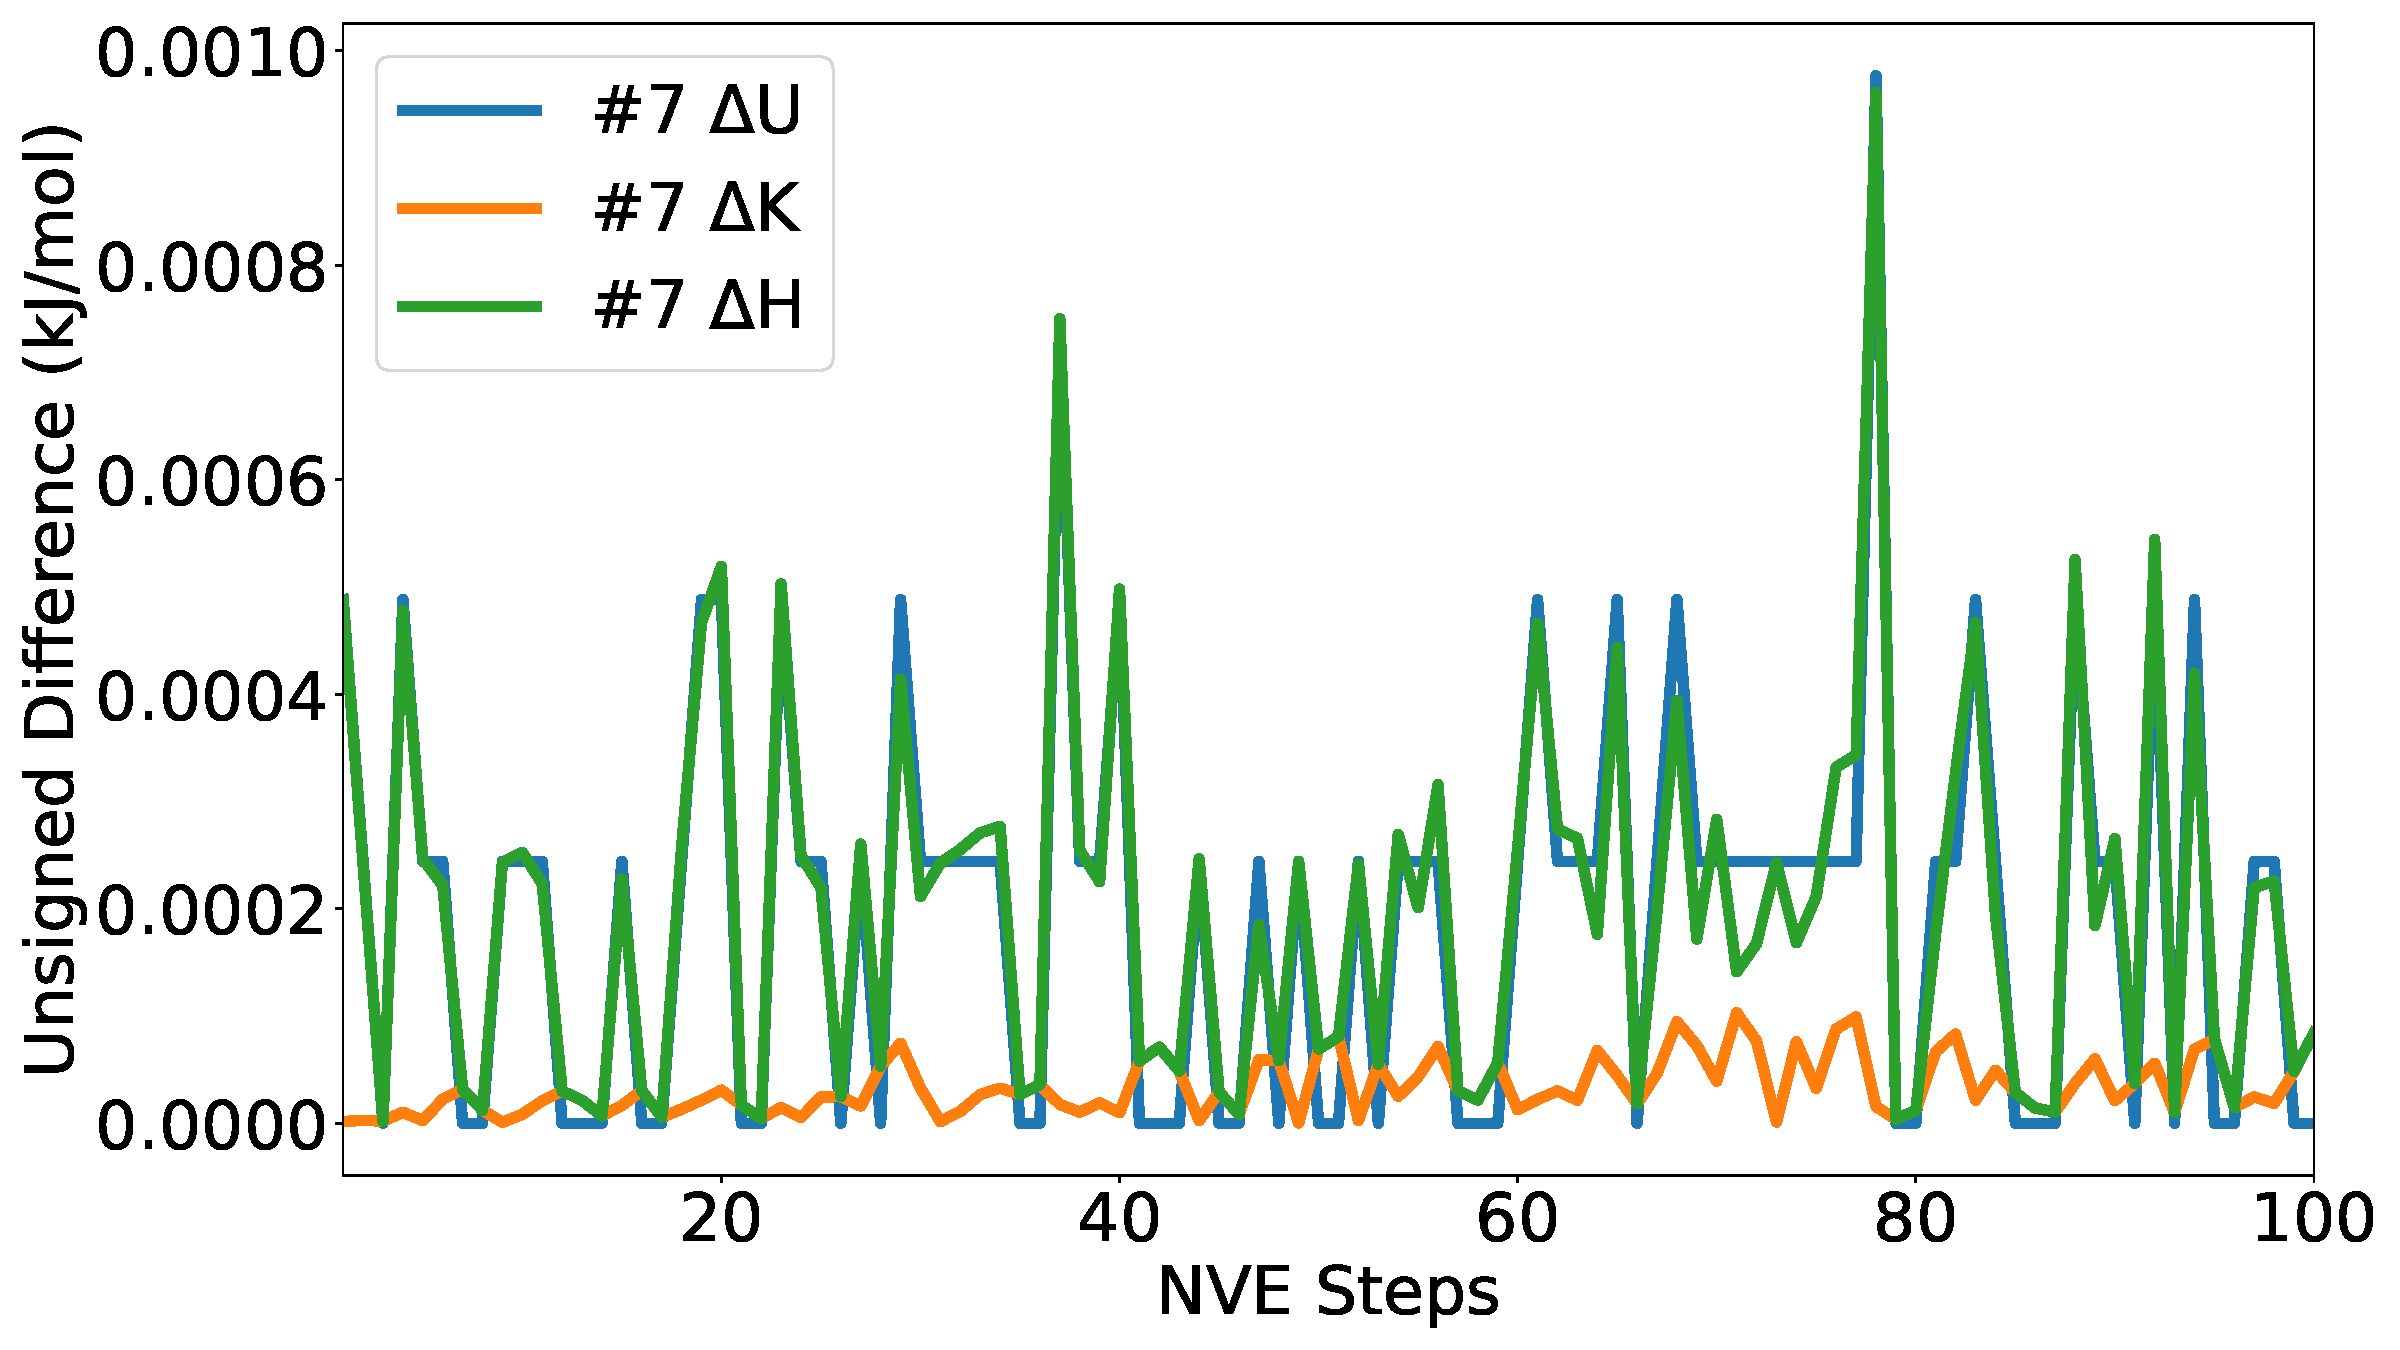
\includegraphics[width=\linewidth]{figs/div7.pdf}
\end{subfigure}
\begin{subfigure}{0.48\textwidth}
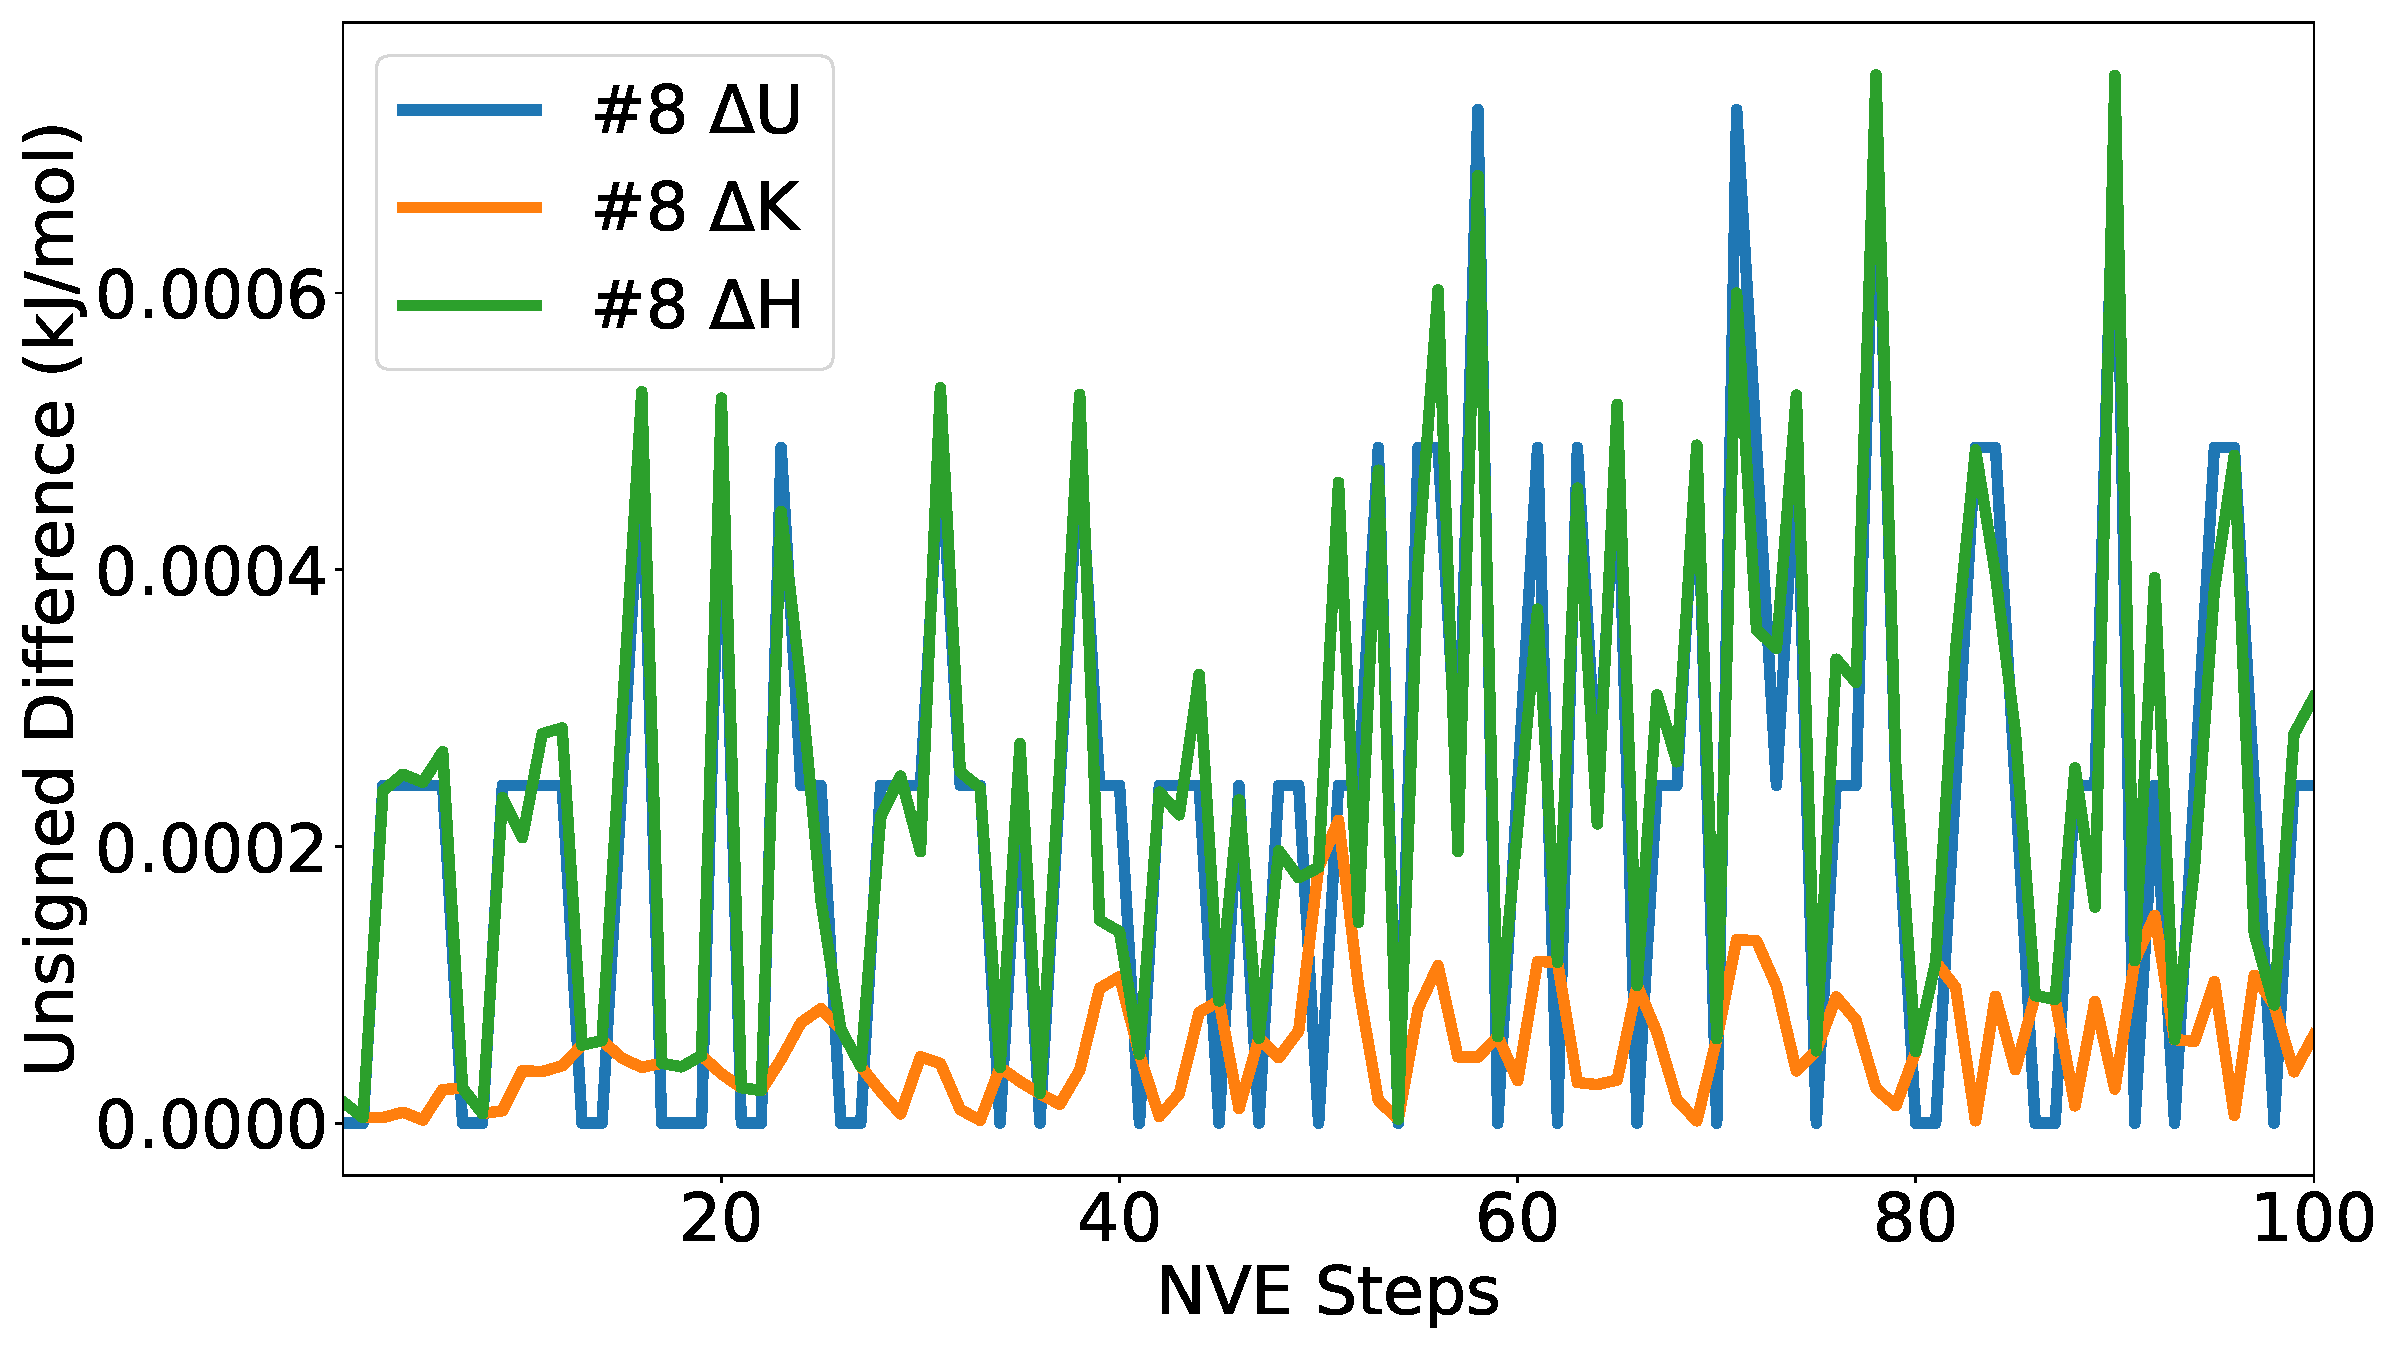
\includegraphics[width=\linewidth]{figs/div8.pdf}
\end{subfigure}
\caption{Comparison of energies across deployment strategies:
unsigned differences in potential energy ($U$), kinetic energy ($K$), and
Hamiltonian ($H$) relative to the baseline simulation over 100 time-steps.
The number in each subfigure indicates the deployment method
as defined in Table~\ref{tb:deploy8}.}\label{fig:convergence}
\end{figure*}
